\section{Design} \label{Design}

The PCAL geometry~\cite{2015002} is shown schematically in Figs.~\ref{fig:S3_1} and \ref{fig:S3_2}. The
active area of PCAL is an isosceles triangle with a base length of $394$~cm and a base angle $\alpha=62.9^\circ$.
The apex of the triangle is nearest the beamline, while a line from the target point to the front face of each
module subtends an angle of $25^\circ$ with respect to the beamline. Each PCAL module is composed of 15
scintillator layers sandwiched with 14 layers of lead, similar to the inner calorimeter of the CLAS EC
\cite{clas6nim}. Each scintillator and lead layer is separated by a $50~\mu$m Teflon sheet and the entire
scintillator/lead volume is confined within a triangular shaped box. Note the EC uses a projective geometry
where each scintillator layer subtends the same solid angle as seen from the target, whereas the PCAL does
not. The PCAL active area is slightly larger than the acceptance of the EC projected towards the CLAS target
to the location of the last layer of the PCAL. 

\begin{figure}[h]
\centering
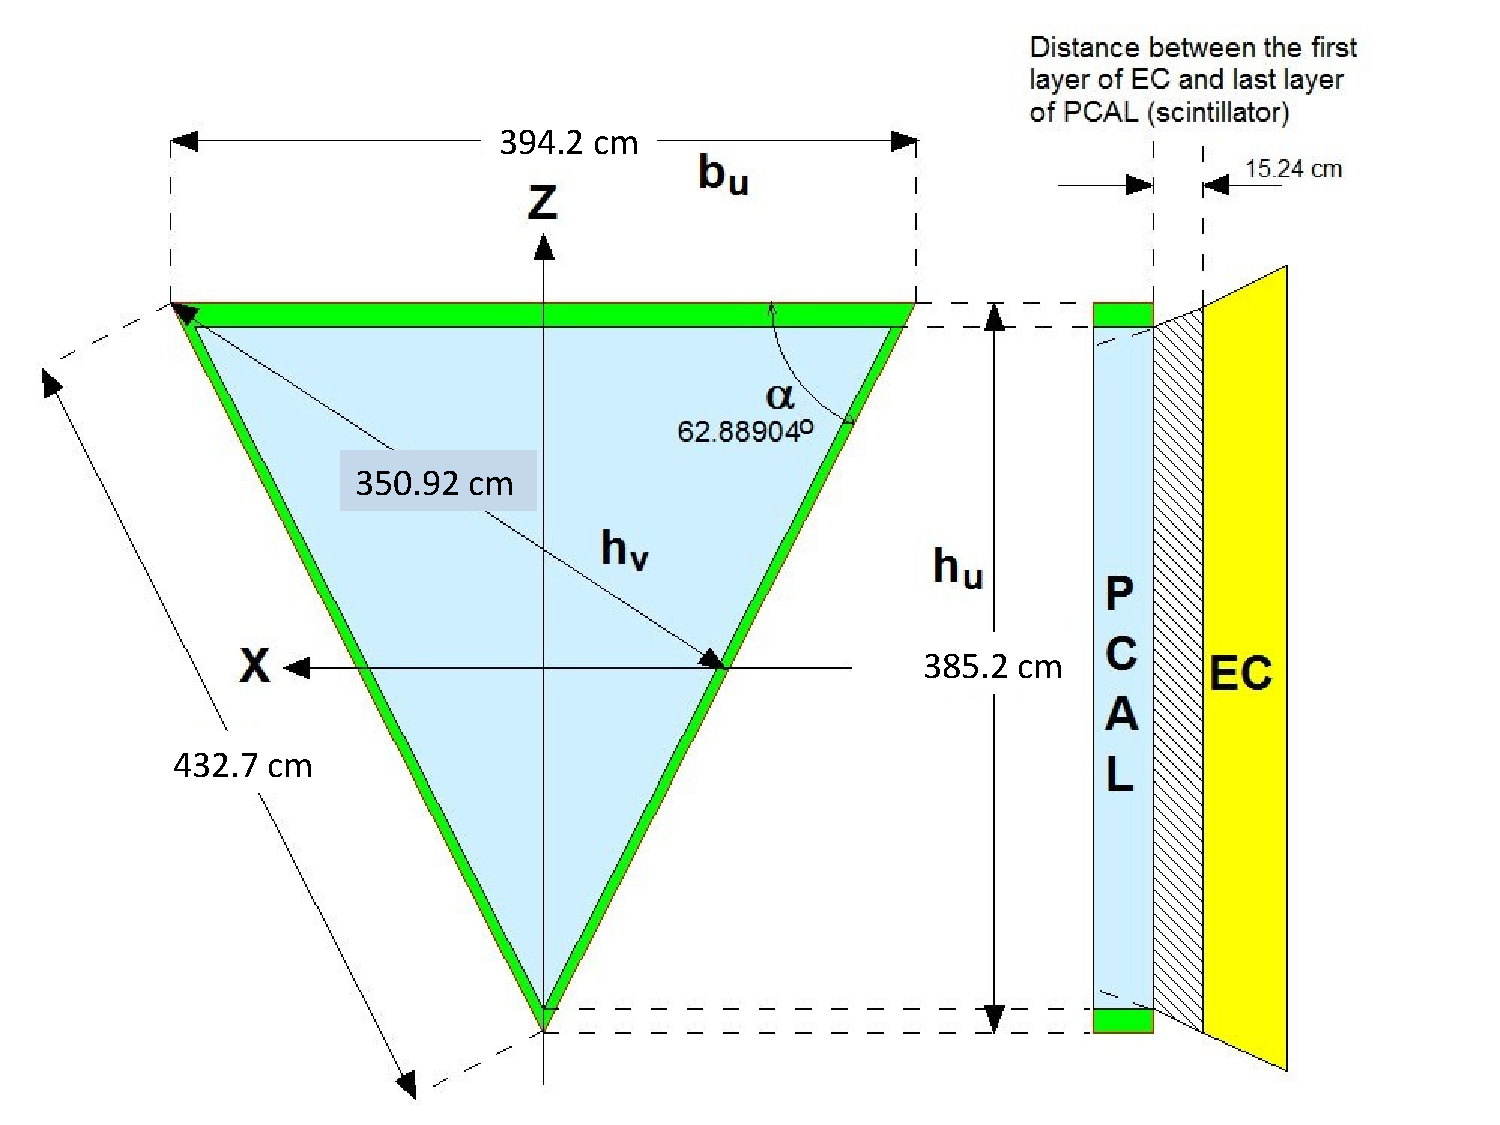
\includegraphics[width=1.0\columnwidth,keepaspectratio]{img/S3_1.pdf}
\caption[Schematic plot of PCAL]{A schematic plot showing the dimensions of a PCAL module. The design length
  $L_1$ of the longest scintillator strips is $L_1=394.2$~cm for the U strips and $L_1=432.7$~cm for the V
  and W strips. }
\label{fig:S3_1}
\end{figure}

The scintillator layers have three alternating stereo readout planes named U, V, and W which are interleaved
with layers of lead as illustrated in Fig.~\ref{fig:S3_2}. The readout planes are divided into scintillator strips
of varying lengths but with a fixed cross-sectional area of $4.5 \times 1$~cm$^2$. In each stereo readout layer
the strips are oriented parallel to one of the sides of the triangle (see Fig.~\ref{fig:S2_2}). For the U-view, the
strips are parallel to the base of the triangle, farthest from the beamline. For the W-view, the strips are parallel
to the U photomultiplier readout side. For the V view, the strips are parallel to the last remaining side.  

\begin{figure}[hbt]
\centering
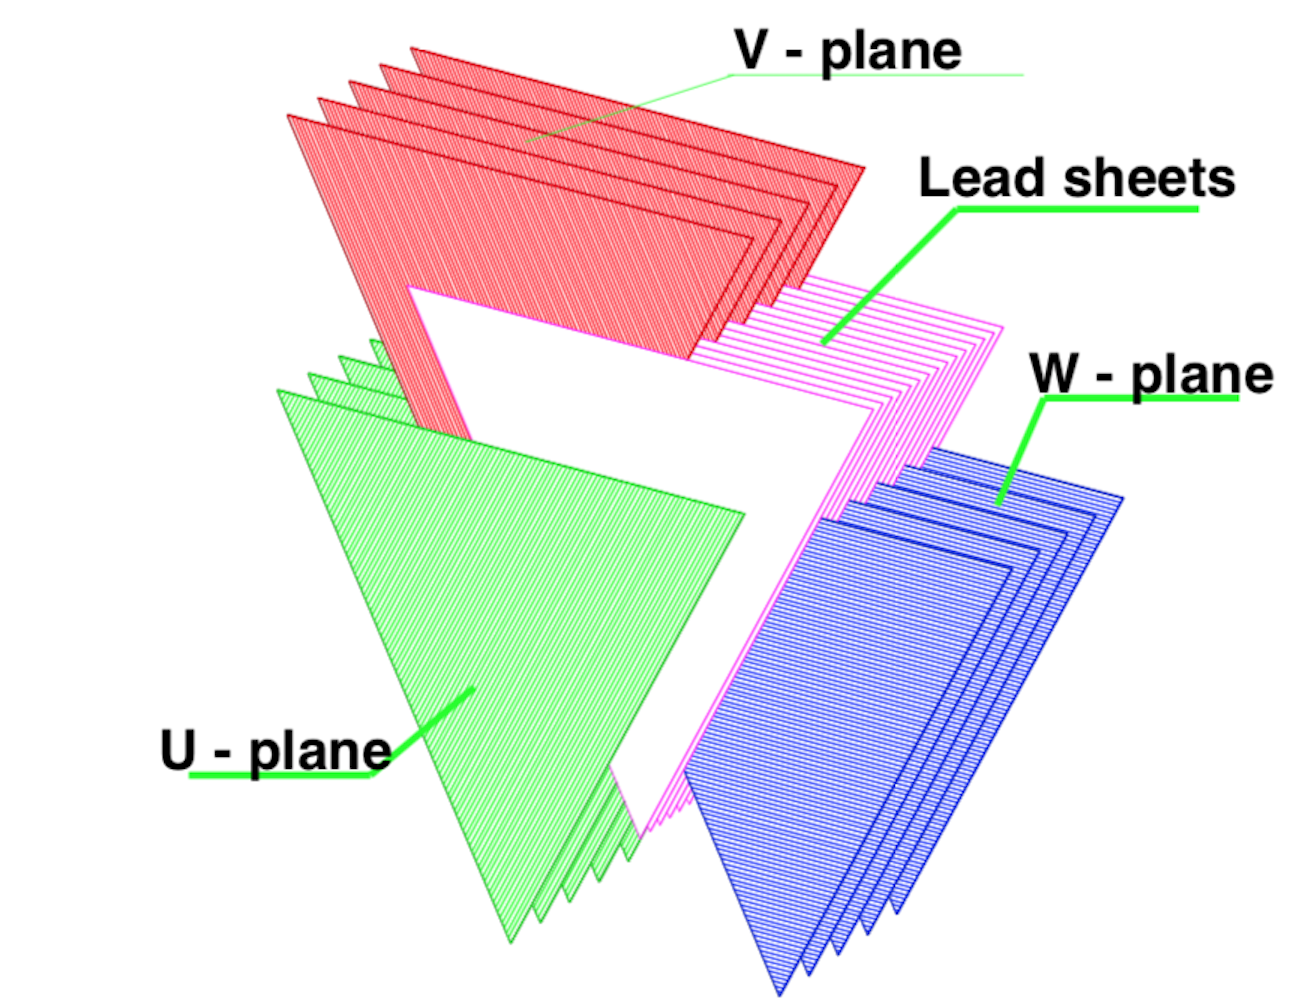
\includegraphics[width=0.95\columnwidth,keepaspectratio]{img/S3_2.png}
\caption[PCAL UVW Layers]{Schematic showing interleaving of U,V,W scintillator layers with lead.}
\label{fig:S3_2}
\end{figure}

Light generated in the scintillator strips by ionizing radiation is wavelength shifted using Kururay Y-11 $1$~mm
diameter multi-clad fibers inserted inside holes running the length of the strips (see Fig.~\ref{fig:S3_4}). The
fibers also transport the light to PMT housing adapters located along the base and U readout side of the triangle.

\begin{figure}[hbt]
\centering
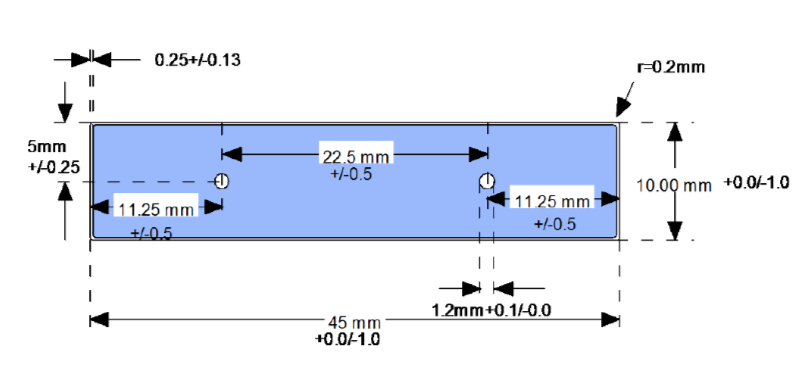
\includegraphics[width=1.05\columnwidth,keepaspectratio]{img/S3_4a.png}
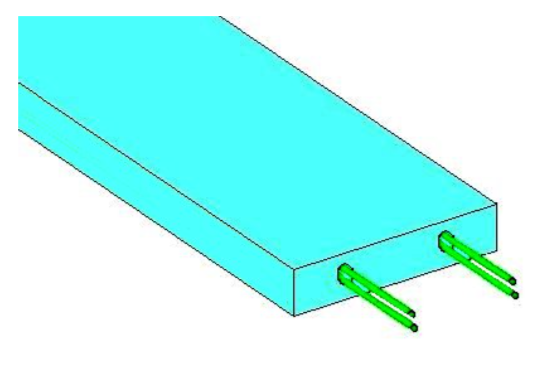
\includegraphics[width=0.75\columnwidth,keepaspectratio]{img/S3_4b.png}
\caption[PCAL UVW Layers]{Top: Design dimensions of the scintillator cross section. Bottom: Rendering of the
  strip with two fibers in each hole.}
\label{fig:S3_4}
\end{figure}

There are $84$ strips in the U-view, and $77$ strips in the V- and W-views. In order to optimize the number of
readout channels, each pair of strips at large scattering angles are combined into a single readout channel (fibers
from two adjacent strips are routed to a single PMT). For the first 52 shortest strips in U and for the last 46
longest strips in the V and W stereo readout planes the 4.5~cm (single strip) segmentation is used. For the
remaining strips, 9.0~cm wide (double strip) segmentation is used. Thus there are a total of 68 PMT readout
channels for U, and 62 for V and W.
